\documentclass[12pt]{article}[margin=1in]
\usepackage{fullpage,graphicx,psfrag,amsmath,amsfonts,verbatim}
\usepackage[small,bf]{caption}
\usepackage{amsthm}
\usepackage{hyperref}
\usepackage{bbm} % for the indicator function to look good
\usepackage{color}
\usepackage{mathtools}
\usepackage{fancyhdr} % for the header
\usepackage{booktabs} % for regression table display (toprule, midrule, bottomrule)
\usepackage{adjustbox} % for regression table display
\usepackage{threeparttable} % to use table notes
\usepackage{natbib} % for bibliography
\input newcommand.tex
\bibliographystyle{apalike}
\setlength{\parindent}{0pt} % remove the automatic indentation

% Settings for page number in the footer
\pagestyle{fancy}
\fancyhf{}
\fancyfoot[C]{\thepage}
\renewcommand{\headrulewidth}{0pt}
\renewcommand{\footrulewidth}{0pt}

\title{\textbf{Demand for Differentiated Products} \\
\vspace{.3cm}
\large Problem Set 1, \\
Empirical Industrial Organization}
\author{Zixuan, Anoosheh, Shuo}
\date{\today}

\begin{document}
\maketitle

\setcounter{page}{1}

\section{Data}
The dataset is a panel of aggregate (model level) car sales along with the
characteristics of each model. The data spans 1977-1981 in the U.S., giving
rise to 5 markets in total. We divide the quantity sold \verb|q| by the market
size (the number of households \verb|hh| in that year) to get the market share
for each model. We also adjust the car price \verb|p| by the consumer price
index \verb|cpi| to get the real price.
\begin{equation*}
    p_{adj} = \frac{100 \times p}{cpi}
\end{equation*}
We rescale the price by $p/1000$ to make the coefficient on price more readable. An overview of the mean and standard deviation of the variables is shown in Table \ref{tab:desc}.

\begin{table}[h!]
    \fontsize{10pt}{12pt}\selectfont
    \centering
    % latex table generated in R 4.3.1 by xtable 1.8-4 package
% Sat Nov  2 19:13:46 2024
\begin{table}[ht]
\centering
\begin{tabular}{rrr}
  \hline
 & mean & sd \\ 
  \hline
dpm & 0.06 & 0.02 \\ 
  door3 & 0.08 & 0.27 \\ 
  door4 & 0.52 & 0.50 \\ 
  door5 & 0.05 & 0.22 \\ 
  at & 0.28 & 0.45 \\ 
  ps & 0.38 & 0.49 \\ 
  air & 0.14 & 0.35 \\ 
  drv & 0.21 & 0.40 \\ 
  wt & 2887.27 & 702.02 \\ 
  hp2wt & 0.36 & 0.08 \\ 
  hp & 104.19 & 34.42 \\ 
  euro & 0.27 & 0.44 \\ 
  japan & 0.14 & 0.34 \\ 
  size & 1.32 & 0.24 \\ 
  wb & 104.47 & 9.14 \\ 
  p & 10.89 & 7.82 \\ 
   \hline
\end{tabular}
\end{table}

    \caption{Descriptive statistics}
    \label{tab:desc}
\end{table}

\section{Logit Model}
\subsection{Utility function}
The standard utility function takes the following linear in characteristics
form:
\begin{equation}
    u_{ij}=X_{j}\beta + \alpha p_{j} + \xi_{j}+ \epsilon_{ij}=\delta_j+\epsilon_{ij}
\end{equation}
where $i$ represents individual and $j$ represents the product. $X_{j}$ includes the following variables: \verb|dpm, door3, door4, door5, at, ps, air, drv, wt, hp2wt, hp, euro, japna, size, wb, (brand dummies)|. We assume that $\epsilon_{ij}$ is distributed type I extreme value and is independent across all products $j$. Thus, the market share for each product is given by (by normalizing the utility of the outside good to zero)
\begin{equation*}
    s_j = \frac{e^{u_{ij}}}{1 + \sum_{k=1}^{J} e^{u_{ik}}}
\end{equation*}
Thus,
\begin{equation}\label{eq:logit}
    \log s_j - \log s_0 = \beta_0 + \beta_1 x_{j1} + \cdots + p_j \alpha + \xi_j
\end{equation}
where $\xi_j$ is the fixed effect/unobserved heterogeneity of each product $j$. For the remaining section, we assume that all characteristics except price are exogenous.

\subsection{Estimation}
The OLS estimation is unbiased and consistent if we assume that $\xi_j$ is
uncorrelated with $p$. We perform two OLS estimations based on equation
\eqref{eq:logit} with and without brand fixed effect. The results are shown in
Table \ref{tab:reg_logit}. However, it is generally not the case. Price is
generally correlated with unobserved characteristics. We construct instruments
based on \citet{berrylevinsohnpakes1995}. That is, for each product
characteristic $x^k$, we compute
\begin{itemize}
    \item $z^k_{j}=\sum_{k\in \mathcal{F}_j, j'\neq j}x^k_{j'}$, the sum of characteristics of all other products belonging to the same firm.
    \item $z^k_{j}=\sum_{k\notin \mathcal{F}_j}x^k_{j'}$, the sum of characteristics of all other products belonging to rival firms.
\end{itemize}
This is a measure of the competitive environment surrounding firms, capturing the substitutability of other available cars to any particular model.

Since we have many $x^k$, we have a large number of instruments. Following
\citet{berrylevinsohnpakes1995}, we selected the following to instrument price
$p$: \verb|const_*, dpm_*, hp2wt_*, size_*, air_*|. The IV estimation results
are shown in Table \ref{tab:reg_logit}.

\subsection{Results}

\begin{table}[h!]
    \fontsize{8pt}{10pt}\selectfont
    \centering
    
\begin{table}[htbp]
   \caption{Logit}
   \centering
   \begin{tabular}{lcccc}
      \tabularnewline \midrule \midrule
      Dependent Variable: & \multicolumn{4}{c}{log(mktshr)-log(shr\_0)}\\
      Estimator & \multicolumn{2}{c}{OLS} & \multicolumn{2}{c}{IV} \\ 
      Model:                       & (1)             & (2)             & (3)                    & (4)\\  
      \midrule
      \emph{Variables}\\
      Constant                     & -5.238$^{***}$  &                 & -5.437$^{***}$         &   \\   
                                   & (1.956)         &                 & (2.023)                &   \\   
      dpm                          & -22.04$^{***}$  & -19.04$^{***}$  & -22.57$^{***}$         & -12.95$^{**}$\\   
                                   & (4.601)         & (3.929)         & (5.125)                & (6.112)\\   
      door3TRUE                    & -0.6235$^{***}$ & -0.5271$^{***}$ & -0.6247$^{***}$        & -0.5444$^{***}$\\   
                                   & (0.2038)        & (0.1876)        & (0.2047)               & (0.1987)\\   
      door4TRUE                    & -0.0636         & -0.0190         & -0.0702                & 0.0479\\   
                                   & (0.1493)        & (0.1344)        & (0.1556)               & (0.1462)\\   
      door5TRUE                    & 0.3424          & 0.4548$^{**}$   & 0.3239                 & 0.5150$^{**}$\\   
                                   & (0.3062)        & (0.2010)        & (0.3163)               & (0.2072)\\   
      at                           & -0.2868         & -0.2917         & -0.3349                & -0.2696\\   
                                   & (0.2102)        & (0.1902)        & (0.2573)               & (0.2107)\\   
      ps                           & 0.2057          & 0.2052          & 0.2072                 & 0.1789\\   
                                   & (0.1738)        & (0.1684)        & (0.1779)               & (0.1946)\\   
      air                          & 0.1226          & -0.1486         & 0.0221                 & 0.5243\\   
                                   & (0.1797)        & (0.1689)        & (0.3451)               & (0.4311)\\   
      drv                          & 0.1029          & 0.1621          & 0.1175                 & 0.2984$^{*}$\\   
                                   & (0.1467)        & (0.1363)        & (0.1491)               & (0.1533)\\   
      wt                           & -0.0022$^{***}$ & -0.0011$^{**}$  & -0.0022$^{***}$        & -0.0012$^{*}$\\   
                                   & (0.0005)        & (0.0004)        & (0.0005)               & (0.0006)\\   
      hp2wt                        & -9.821$^{***}$  & -5.934$^{**}$   & -9.975$^{***}$         & -8.677$^{**}$\\   
                                   & (3.242)         & (2.356)         & (3.046)                & (3.761)\\   
      hp                           & 0.0381$^{***}$  & 0.0228$^{**}$   & 0.0371$^{***}$         & 0.0410$^{**}$\\   
                                   & (0.0112)        & (0.0088)        & (0.0111)               & (0.0163)\\   
      euro                         & -1.772$^{***}$  &                 & -1.938$^{***}$         &   \\   
                                   & (0.2136)        &                 & (0.5001)               &   \\   
      japan                        & -0.1290         &                 & -0.1618                &   \\   
                                   & (0.2246)        &                 & (0.2413)               &   \\   
      size                         & 2.710$^{***}$   & 0.6433          & 2.750$^{***}$          & 0.7661\\   
                                   & (0.9020)        & (0.9060)        & (0.8873)               & (1.191)\\   
      wb                           & 0.0224          & 0.0431$^{*}$    & 0.0265                 & 0.0171\\   
                                   & (0.0234)        & (0.0254)        & (0.0263)               & (0.0342)\\   
      p                            & -0.0396$^{***}$ & -0.0644$^{***}$ & -0.0213                & -0.1950$^{**}$\\   
                                   & (0.0126)        & (0.0179)        & (0.0526)               & (0.0758)\\   
      \midrule
      \emph{Fixed-effects}\\
      firmids                      &                 & Yes             &                        & Yes\\  
      \midrule
      \emph{Fit statistics}\\
      Observations                 & 501             & 501             & 501                    & 501\\  
      Adjusted R$^2$               & 0.63354         & 0.72408         & 0.63070                & 0.67282\\  
      Wald (1st stage), p          &                 &                 & 4.6332                 & 7.1002\\  
      Wald (1st stage), p-value, p &                 &                 & 0.00112                & $1.48\times 10^{-5}$\\   
      Sargan                       &                 &                 & 56.889                 & 2.6361\\  
      Sargan, p-value              &                 &                 & $2.71\times 10^{-12}$  & 0.45119\\  
      \midrule \midrule
      \multicolumn{5}{l}{\emph{Clustered (modelid) standard-errors in parentheses}}\\
      \multicolumn{5}{l}{\emph{Signif. Codes: ***: 0.01, **: 0.05, *: 0.1}}\\
   \end{tabular}
\end{table}



    \caption{Logit estimation results}
    \label{tab:reg_logit}
\end{table}

We observe that the coefficient on price, $\alpha$, is larger (in absolute
terms) but noisily estimated using IV compared to OLS. This makes sense as the
simple OLS regression yields downward-biased estimates (in terms of magnitude)
because failing to account for endogeneity underestimates the effect of price
on market share.

\section{Nested Logit Model}
\subsection{Utility function}
We relax the assumption that $\varepsilon_{ij}$ is independent across $j$.
Instead, we group the products into nests based on their size. The 3 nests are
\verb|compact, midsize, large| plus one outside option. Now the utility
function is given by
\begin{equation}
    \begin{split}
        u_{ij} & =X_{j}\beta + \alpha p_{j} + \xi_{j} + \eta_{ig} + \epsilon_{ij} \\
               & =\delta_j + \eta_{ig} + (1 - \sigma)\epsilon_{ij}
    \end{split}
\end{equation}
Following the derivation in \citet{berry1994estimating}, the estimation equation is
\begin{equation}
    \log(s_j) - \log(s_0) = x_j\beta + p_j\alpha + \sigma\log(\bar{s}_{j|g}) + \xi_j
\end{equation}

\subsection{Estimation}
In addition to $p$, $\log(\bar{s}_{j|g})$ is also endogenous. We follow
\citet{berry1994estimating} to construct additional instruments for
$\log(\bar{s}_{j|g})$, which is the sum of product characteristics of the rival
firms in the same nest $g$. We exploit the competition posed by rivals with the
added feature of this `competition' coming from within the same group (i.e.
size category). The results from demand estimation are presented in Table
\ref{tab:reg_nested_logit}.

\subsection{Results}

\begin{table}[h!]
    \fontsize{8pt}{10pt}\selectfont
    \centering
    
\begin{table}[htbp]
   \caption{Logit}
   \centering
   \begin{tabular}{lcccc}
      \tabularnewline \midrule \midrule
      Dependent Variable: & \multicolumn{4}{c}{log(mktshr)-log(shr\_0)}\\
      Estimator & \multicolumn{2}{c}{OLS} & \multicolumn{2}{c}{IV} \\ 
      Model:                                     & (1)             & (2)                    & (3)                    & (4)\\  
      \midrule
      \emph{Variables}\\
      Constant                                   & -4.712$^{***}$  &                        & -4.612$^{***}$         &   \\   
                                                 & (0.8660)        &                        & (1.232)                &   \\   
      dpm                                        & -8.137$^{***}$  & -9.190$^{***}$         & -12.36$^{***}$         & -17.52$^{**}$\\   
                                                 & (1.616)         & (1.561)                & (2.926)                & (6.855)\\   
      door3TRUE                                  & -0.0134         & 0.0662                 & -0.2306$^{**}$         & -0.7178$^{**}$\\   
                                                 & (0.0658)        & (0.0602)               & (0.1142)               & (0.3026)\\   
      door4TRUE                                  & -0.0311         & 0.0031                 & -0.0332                & 0.0236\\   
                                                 & (0.0569)        & (0.0511)               & (0.0791)               & (0.1726)\\   
      door5TRUE                                  & 0.1019          & 0.1758$^{**}$          & 0.2151                 & 0.5828$^{**}$\\   
                                                 & (0.0988)        & (0.0717)               & (0.1609)               & (0.2868)\\   
      at                                         & 0.0367          & -0.0741                & -0.0094                & -0.3407\\   
                                                 & (0.0969)        & (0.1086)               & (0.1263)               & (0.2534)\\   
      ps                                         & -0.1059         & -0.0123                & 0.0038                 & 0.2511\\   
                                                 & (0.0983)        & (0.1127)               & (0.1090)               & (0.2241)\\   
      air                                        & 0.0162          & -0.0004                & 0.2007                 & 0.3021\\   
                                                 & (0.0748)        & (0.0836)               & (0.1452)               & (0.3997)\\   
      drv                                        & 0.1261$^{**}$   & 0.0432                 & 0.0964                 & 0.2981\\   
                                                 & (0.0498)        & (0.0515)               & (0.0814)               & (0.1983)\\   
      wt                                         & -0.0003         & $-5.32\times 10^{-5}$  & -0.0009$^{**}$         & -0.0015$^{*}$\\   
                                                 & (0.0003)        & (0.0002)               & (0.0004)               & (0.0008)\\   
      hp2wt                                      & -1.955          & -1.307                 & -4.554$^{*}$           & -9.340$^{**}$\\   
                                                 & (1.468)         & (1.202)                & (2.487)                & (4.550)\\   
      hp                                         & 0.0104$^{**}$   & 0.0066                 & 0.0219$^{***}$         & 0.0411$^{**}$\\   
                                                 & (0.0052)        & (0.0046)               & (0.0083)               & (0.0187)\\   
      euro                                       & -0.1817$^{*}$   &                        & -0.5101$^{*}$          &   \\   
                                                 & (0.0977)        &                        & (0.2800)               &   \\   
      japan                                      & 0.0878          &                        & 0.0579                 &   \\   
                                                 & (0.0836)        &                        & (0.1300)               &   \\   
      size                                       & 1.691$^{***}$   & 1.059$^{**}$           & 1.998$^{***}$          & 0.6089\\   
                                                 & (0.4538)        & (0.4710)               & (0.5905)               & (1.259)\\   
      wb                                         & 0.0003          & 0.0107                 & 0.0022                 & 0.0336\\   
                                                 & (0.0111)        & (0.0112)               & (0.0151)               & (0.0371)\\   
      p                                          & -0.0165$^{***}$ & -0.0142                & -0.0516$^{**}$         & -0.1755$^{**}$\\   
                                                 & (0.0058)        & (0.0095)               & (0.0230)               & (0.0768)\\   
      log(mktshr\_g)                             & 0.8896$^{***}$  & 0.8759$^{***}$         & 0.5704$^{***}$         & -0.2627\\   
                                                 & (0.0256)        & (0.0285)               & (0.0808)               & (0.2987)\\   
      \midrule
      \emph{Fixed-effects}\\
      firmids                                    &                 & Yes                    &                        & Yes\\  
      \midrule
      \emph{Fit statistics}\\
      Observations                               & 501             & 501                    & 501                    & 501\\  
      Adjusted R$^2$                             & 0.93445         & 0.94171                & 0.88957                & 0.54513\\  
      Wald (1st stage), p                        &                 &                        & 4.0649                 & 5.2015\\  
      Wald (1st stage), log(mktshr\_g)           &                 &                        & 8.5635                 & 4.1898\\  
      Wald (1st stage), p-value, p               &                 &                        & 0.00011                & $3\times 10^{-6}$\\   
      Wald (1st stage), p-value, log(mktshr\_g)  &                 &                        & $6.31\times 10^{-11}$  & $7.27\times 10^{-5}$\\   
      Sargan                                     &                 &                        & 132.03                 & 12.690\\  
      Sargan, p-value                            &                 &                        & $4.8\times 10^{-26}$   & 0.04824\\  
      \midrule \midrule
      \multicolumn{5}{l}{\emph{Clustered (modelid) standard-errors in parentheses}}\\
      \multicolumn{5}{l}{\emph{Signif. Codes: ***: 0.01, **: 0.05, *: 0.1}}\\
   \end{tabular}
\end{table}



    \caption{Nested Logit estimation results}
    \label{tab:reg_nested_logit}
\end{table}

\paragraph{Price $\alpha$} Once again, the OLS estimates of $\alpha$ are biased towards zero. The OLS
estimation is upward biased.

\paragraph{Within nest substitutability $\hat{\sigma}$} The estimate of $\sigma$ is smaller in IV than in OLS, suggesting a lower degree of intra-group substitutability once we have accounted for the endogeneity of prices and within-group shares.

\paragraph{Instrument test}
%Zixuan:
The F-test of the first stage is a weak instrument test. The null hypothesis is
that the instruments are weak, which is rejected by the test, implying that our
instruments are not too weak. The Sargan-Hansen test is a test of
over-identification. The null hypothesis is that all instruments are valid,
which is rejected by the test, implying that some instruments are not suitable.

%Anoosheh:
From the results of the test of overidentifying restrictions, we are able to
reject the null that \textit{all} instruments are valid. Our instruments also
appear to be weak as indicated by the conditional likelihood ratio (CLR) test
for weak IV-robustness (for an over-identified system). We cannot reject the
joint null of $H_0: \alpha=0, \; \sigma=0$. \\ This could point to a possible
failure of the exogeneity of the instruments we use.

\section{Random Coefficients Model}
\subsection{Utility function}
Next, we turn to our final specification of a random-coefficients model \`a la
\citet{berrylevinsohnpakes1995} where indirect utility is defined as
\begin{equation}
    u_{ij}=X_{j}\beta + \alpha p_{j} + \xi_{j} + \eta_i\text{size}_j + \epsilon_{ij} = \delta_j + \eta_i\text{size}_j + \epsilon_{ij}
\end{equation}
where $\eta_i \sim N(0,\sigma^2)$.
The difference here is that the coefficient $\eta_i$ is allowed to vary across
households $i$. After refactoring the indirect utility, we arrive at the
following expression, where the last line arises since we have learned that
$\bar{\eta}$ is zero. So that, even if the $\epsilon_{ij}$'s are still i.i.d.
TIEV across $j$, the composite error is not.

Now, the aggregate market share becomes
\[
    s_j = \int \frac{\exp{(\delta_j + \eta_i \text{Size}_j)}}{1 + \sum_{j^{\prime}}^{J} \exp{(\delta_{j^{\prime}} + \eta_i \text{Size}_{j^{\prime}})}} dF(\eta_i)
\]

\subsection{Estimation}
Unlike before, the relationship between $\log(s_j)$ and $\delta_j$ is no longer
as explicit. We need to find a way to recover $\delta_j$ from the observed
market share $s_j$. We follow the method provided by
\citet{berrylevinsohnpakes1995}. The procedure involves several steps,
including drawing values from a normal distribution, contraction mapping, and
GMM estimation.

The procedure is the following:
\begin{enumerate}
    \item We draw 500 values from a normal distribution $N(0,1)$.
    \item We pick an initial value of $\sigma$.
    \item Given a value of $\sigma$, we calculate the predicted market share based on
          $\sigma$ by approximate the following integral
          \begin{equation*}
              s_j(\delta_1,\ldots,\delta_j)=\int \frac{e^{\delta_j+\eta_i\text{size}_j}}{1+\sum_{k=1}^{J}e^{\delta_k+\eta_i\text{size}_k}}dF(\eta_i)
          \end{equation*}
    \item We use contraction mapping to find the value of $\delta$ vector that makes the
          predicted market share equal to the observed market share.
    \item Once we have the $\delta$ vector which is linear in $X$.
          \begin{equation*}
              \delta_j=X_j\beta+\alpha p_j+\xi_j
          \end{equation*}
          We can estimate the $\beta$ and $\alpha$ with some instruments, thus getting the residual $\xi_j$.
    \item We compute the empirical moment condition is $Q(\sigma)=Z'\xi$ where $Z$ is the
          instruments and $\xi$ is the residual, which is of dimension $ \# \text{instr}
              \times 1$. The GMM objective function is thus $Q(\sigma)'WQ(\sigma)$.
          \begin{equation*}
              \min_{\sigma} Q(\sigma)'WQ(\sigma)
          \end{equation*}
\end{enumerate}

Note that by creating nests, we create a new endogenous variable
$\log(\bar{s}_{j|g})$ for which we create new instruments. Similarly, by
creating a random coefficient term $\eta_i$ on size, we create extra
endogeneity. (How so?) We follow \citet{gandhihoude2019measuring} to construct
extra differentiation instrument.
\begin{enumerate}
    \item Quadratic: $\sum_{j' \neq j} (d_{j'j}^k)^2$ where $d_{j'j}^k$ is the distance
          between product $j$ and $j'$ in characteristic $k$.
    \item Local: $\sum_{j' \neq j} 1\{d_{j'j}^k < sd^k\}$ where $sd^k$ is the standard
          deviation of $x^k$ acorss all markets.
\end{enumerate}
We select the following instruments in addition to the previous nested logit
instruments: \verb|size_local, disp_local, wb_local, hp_local, hp2wt_local|.

\subsection{Results}
We plot the GMM objective function w.r.t. $\sigma$ in Figure
\ref{fig:iv_local_diff}.

\begin{figure}[h!]
    \centering
    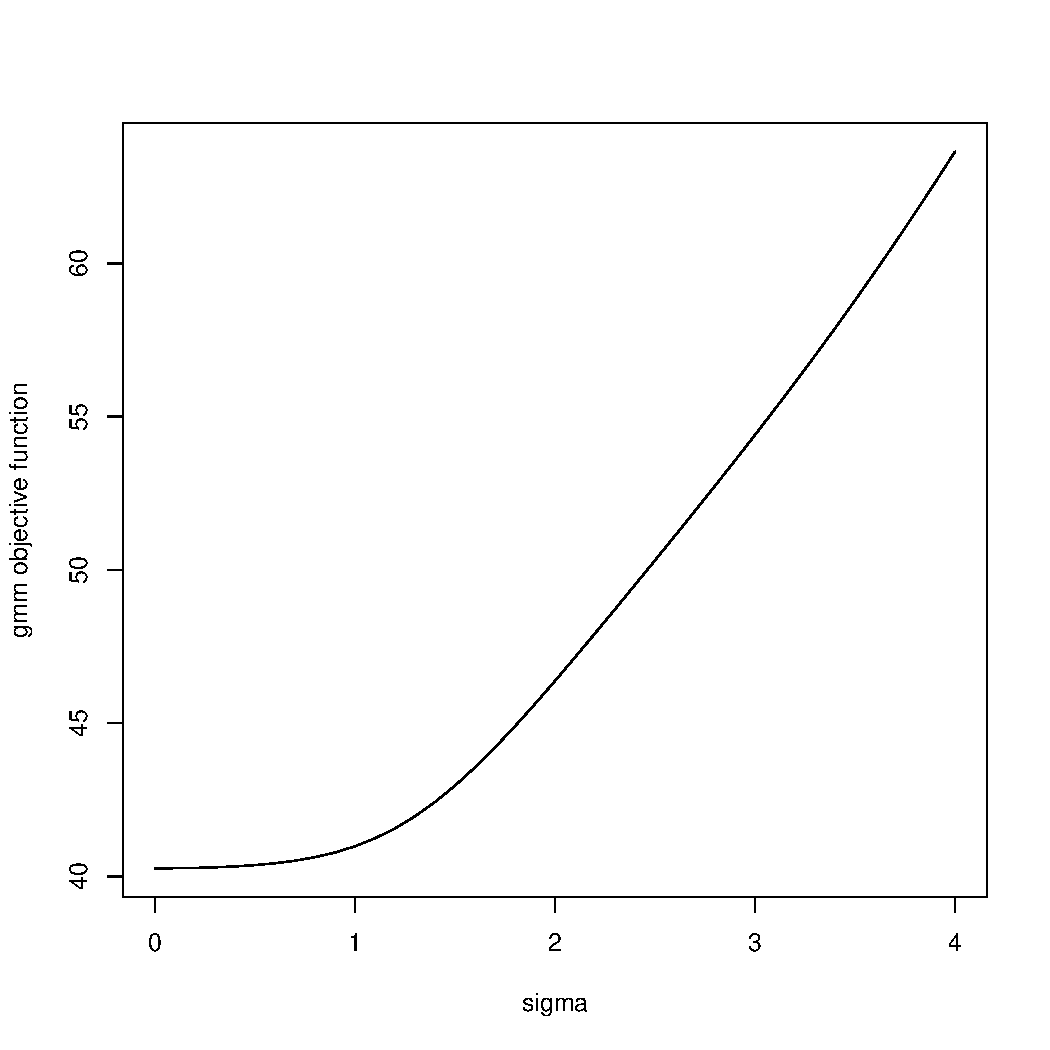
\includegraphics[width=0.8\textwidth]{../Results/Figures/gmm_obj_iv_local.pdf}
    \caption{GMM objective function w.r.t. $\sigma$}
    \label{fig:iv_local_diff}
\end{figure}

The sigma that minimizes the GMM objective function is 2.3. Given the
$\hat{\sigma}$, we recover the mean utility $\delta_j$ for each product in
every market. The estimation results by regressing $\delta_j$ on $X_j$ and
$p_j$ are shown in Table \ref{tab:reg_rand_coef}.

\begin{table}[h!]
    \fontsize{10pt}{12pt}\selectfont
    \centering
    
\begingroup
\centering
\begin{tabular}{lc}
   \tabularnewline \midrule \midrule
   Dependent Variable:            & y\\  
   Model:                         & (1)\\  
   \midrule
   \emph{Variables}\\
   Constant                       & -1.741\\   
                                  & (1.938)\\   
   p                              & -0.0870$^{**}$\\   
                                  & (0.0428)\\   
   dpm                            & -20.46$^{***}$\\   
                                  & (5.398)\\   
   door3TRUE                      & -0.6440$^{***}$\\   
                                  & (0.2082)\\   
   door4TRUE                      & -0.0094\\   
                                  & (0.1522)\\   
   door5TRUE                      & 0.4822\\   
                                  & (0.3175)\\   
   at                             & -0.2956\\   
                                  & (0.2242)\\   
   ps                             & 0.2206\\   
                                  & (0.1728)\\   
   air                            & 0.5580$^{*}$\\   
                                  & (0.2874)\\   
   drv                            & 0.0961\\   
                                  & (0.1538)\\   
   wt                             & -0.0023$^{***}$\\   
                                  & (0.0006)\\   
   hp2wt                          & -10.12$^{***}$\\   
                                  & (3.726)\\   
   hp                             & 0.0421$^{***}$\\   
                                  & (0.0134)\\   
   euro                           & -1.212$^{***}$\\   
                                  & (0.4153)\\   
   japan                          & 0.0573\\   
                                  & (0.2280)\\   
   wb                             & -0.0207\\   
                                  & (0.0225)\\   
   \midrule
   \emph{Fit statistics}\\
   Observations                   & 501\\  
   Adjusted R$^2$                 & 0.69806\\  
   F-test (1st stage), p          & 4.6944\\  
   F-test (1st stage), p-value, p & $2.99\times 10^{-7}$\\   
   Sargan                         & 72.714\\  
   Sargan, p-value                & $3.71\times 10^{-11}$\\   
   \midrule \midrule
   \multicolumn{2}{l}{\emph{Clustered (modelid) standard-errors in parentheses}}\\
   \multicolumn{2}{l}{\emph{Signif. Codes: ***: 0.01, **: 0.05, *: 0.1}}\\
\end{tabular}
\par\endgroup



    \caption{Random coefficient on size}
    \label{tab:reg_rand_coef}
\end{table}

\section{Markups and Merger Simulation}
\subsection{Price setting equation}
The profit of a multiproduct firm is
\begin{equation*}
    \Pi_f = \sum_{j\in \mathcal{J}_f} (p_j - c_j) s_j M
\end{equation*}
since $s_j M$ represents the sales of product $j$. The optimal price is given by taking the first order derivative with respect to $p$:
\begin{equation*}
    s_j + \sum_{k\in \mathcal{J}_f} \frac{\partial s_k}{\partial p_j} (p_k - c_k) = 0 \quad \forall j \in \mathcal{J}_f
\end{equation*}
The first term is the direct impact of changing $p_j$. The second term is the
impact on the profits of other products of the firm.
For firm $f$, the pricing equation written in matrix form gives:
\begin{equation*}
    S^f + \Omega^f (P^f - C^f) = 0
\end{equation*}
where $\Omega^f$ is the matrix of cross-price elasticities.
For example, if firm $f$ has two products, the matrix is $$
    \Omega^f =\begin{bmatrix}
        \frac{\partial s_1}{\partial p_1} & \frac{\partial s_1}{\partial p_2} & 0 \\\ \frac{\partial s_2}{\partial p_1} &\frac{\partial s_2}{\partial p_2} & 0 \\0 & 0 &0\\
    \end{bmatrix}$$
Therefore, aggregate the pricing equation for all firms, we have $$ S + \Omega
    \odot O (P-C) = 0 $$ where $O$ is the ownership matrix.
We take $\hat{\alpha} = -0.087$. We estimate marginal cost (negative), markup,
and elasticity for each year. We simulate a merger between firm 17 and firm 7
by modifying the ownership matrix. The mean results are shown in Table
\ref{tab:post_merger_mean}.

\begin{table}[h!]
    \fontsize{10pt}{12pt}\selectfont
    \centering
    % latex table generated in R 4.2.1 by xtable 1.8-4 package
% Sat Nov  2 15:53:35 2024
\begin{table}[ht]
\centering
\begin{tabular}{rrrrrrr}
  \hline
 & year & p & mc & mk & elas & p\_new \\ 
  \hline
1 & 1977 & 9.89 & -2.73 & 12.62 & -124.46 & 9.89 \\ 
  2 & 1978 & 10.67 & -1.95 & 12.61 & -134.01 & 10.67 \\ 
  3 & 1979 & 10.50 & -2.06 & 12.56 & -131.42 & 10.50 \\ 
  4 & 1980 & 10.71 & -1.82 & 12.53 & -133.78 & 10.71 \\ 
  5 & 1981 & 12.42 & -0.06 & 12.48 & -154.55 & 12.42 \\ 
   \hline
\end{tabular}
\label{tab:post_merger_mean}
\end{table}

    \caption{Markup}
    \label{tab:post_merger_mean}
\end{table}
The anomaly is that we get
negative marginal cost, this is due to the small $\hat{\alpha}$ from the
estimation. Also, the effect of average price seems to be very insignificant.

\subsection{Estimation}
We calculate consumer surplus pre- and post-merger in monetary terms:
\begin{equation*}
    CS_i = E(\max_j u_{ij}) = \frac{\ln(1 + \sum_j \exp(\delta_j + \mu_{ij}))}{\alpha_i}
\end{equation*}
Thus in total:
\begin{equation*}
    CS = M \int CS_i(\theta) dF(\theta)
\end{equation*}

The result is shown in Table \ref{tab:post_merger_cs}.
\begin{table}[h!]
    \fontsize{10pt}{12pt}\selectfont
    \centering
    % latex table generated in R 4.3.1 by xtable 1.8-4 package
% Sat Nov  2 19:16:50 2024
\begin{table}[ht]
\centering
\begin{tabular}{rrrrrrrr}
  \hline
 & year & nb\_hh & shr\_0 & shr\_0\_new & cs\_pre & cs\_post & diff \\ 
  \hline
1 & 1977 & 74142 & 0.88 & 0.92 & 113392.09 & 74255.59 & -39136.50 \\ 
  2 & 1978 & 76030 & 0.88 & 0.91 & 109959.37 & 84723.89 & -25235.48 \\ 
  3 & 1979 & 77330 & 0.89 & 0.92 & 99446.89 & 72200.37 & -27246.52 \\ 
  4 & 1980 & 80776 & 0.91 & 0.94 & 88677.33 & 59681.78 & -28995.55 \\ 
  5 & 1981 & 82368 & 0.91 & 0.93 & 86013.23 & 64848.35 & -21164.88 \\ 
   \hline
\end{tabular}
\end{table}

    \caption{Consumer surplus}
    \label{tab:post_merger_cs}
\end{table}

\pagebreak
\newpage
\bibliography{../References/ref.bib}

\end{document}